% !TEX root = ../thesis-example.tex
%
\chapter{Multiple time series forecasting using quasi-randomized functional link neural networks}
\label{sec:rvfl_mts}

\section{Introduction}

In this chapter, we are interested in obtaining forecasts for multiple time series, by taking into account the potential nonlinear relationships between their observations. This type of problem has been tackled recently by \cite{exterkate2016nonlinear}, who applied kernel regularized least squares to a set of macroeconomic time series. The Long Short-Term Memory neural networks (LSTM) architectures (introduced by \cite{hochreiter1997long}) are another family of models, which are currently widely used for this purpose. As a basis for our model, we will use (quasi-)randomized neural networks known as Random Vector Functional Link neural networks (RVFL networks hereafter)

\medskip

The forecasting method described in this chapter, provides useful inputs for Insurance quantitative Risk Management models; the interested reader can refer to \cite{bonnin2015retraite} for example.

\medskip

To the best of our knowledge, randomized neural networks were introduced by \cite{schmidt1992feedforward}, and the RVFL networks were introduced by \cite{pao1994learning}. An early approach for multivariate time series forecasting using neural networks is described in \cite{chakraborty1992forecasting}. They applied a \textit{back propagation} algorithm from \cite{rumelhart1988learning} to trivariate time series, and found that the combined training of the series gave better forecasts than a separate training of each individual series. The novelty of the approach described in this chapter is to derive an RVFL model for multiple time series, under two separate regularization constraints on the parameters, as it will be described in details in  section ~\ref{solve_rvfl}.

\medskip

RVFL networks are \textit{multilayer feedforward} neural networks, in which there is a \textit{direct link} between the predictors and the output variable, aiming at capturing the linear relationships. In addition to the \textit{direct link}, there are new features: the hidden nodes (the dataset is augmented), that help to capture the nonlinear relationships between the time series. These new features are obtained by random simulation over a given interval. More details on the \textit{direct link} and the hidden nodes will be provided in the next section.

\medskip

The RVFL networks have been successfully applied to solving different types of classification and regression problems; see for example \cite{dehuri2010comprehensive}. More specifically, they have been applied to univariate time series forecasting by \cite{ren2016random}. A comprehensive survey can be found in \cite{zhang2016comprehensive}; where a large number of model specifications are tested on classification problems, including changing the range of hidden layer's randomization.

\medskip

Here, we will use RVFL networks with one hidden layer. And instead of relying on fully randomized nodes, we will use sequences of deterministic quasi-random numbers. Indeed, with fully randomized nodes, the model fits obtained are dependent on the choice of a simulation \textit{seed}. Typically, a different fitting solution would be obtained for each \textit{seed}.

\medskip

In our various numerical examples from section \ref{sec:numericalexamples}, we will apply the RVFL networks to forecasting trivariate time series, notably (but not only) in a Dynamic Nelson Siegel (DNS) framework (see \cite{nelson1987parsimonious}, \cite{diebold2006forecasting}). We will obtain point forecasts and predictive distributions  for the series, and see that in this RVFL framework, one (or more) variable(s) can be stressed, and influence the others. More precisely, about this last point, it means that it is possible, as in dynamic regression models (\cite{pankratz2012forecasting}) to assign a specific future value to one regressor, and obtain forecasts of the remaining variables. Another advantage of the model described here, is its ability to integrate multiple other exogenous variables, without overfitting in-sample data.

\section{Description of the model}

The general procedure for obtaining the model's optimal parameters and predictions is  summarized in figure \ref{fig:flowchart}. 

\begin{figure}[!htb]
\centering
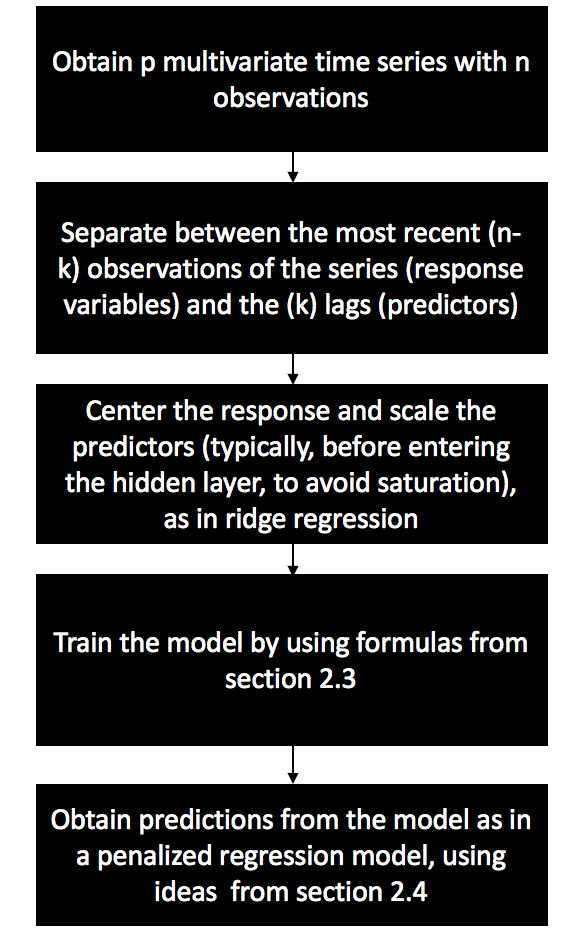
\includegraphics[width=5.5cm]{gfx/chapter-rvfl-mts/flowchart}
\caption{}
\label{fig:flowchart}
\end{figure}


This procedure is described in details in the next sections, especially sections \ref{solve_rvfl} and \ref{sec:preds}. 

\clearpage

\subsection{On a single layer RVFL networks}
\label{sec:modeldesc}

We rely on single layer feed forward neural networks (SLFN).
Considering that an output variable $y \in \RR^n$ is to be explained by a set of observed predictors $Z^{(j)} \in \RR^n$, $j \in \left\lbrace 1, \ldots,
p\right\rbrace$, the RVFL networks we will use to explain $y$ can be described for $i \in \left\lbrace 1, \ldots, n\right\rbrace$ as:
$$
y_i = \beta_0 + \sum_{j = 1}^p \beta_j Z_i^{(j)} + \sum_{l = 1}^L \gamma_l \:
g\left(\sum_{j = 1}^p W^{(j, l)} Z_i^{(j)}\right) + \epsilon_i
$$

\medskip

$g$ is called \textit{activation function}, $L$ is the number of nodes in the hidden
layer, $W^{(j, l)}$ are elements of the hidden layer, and the parameters
$\beta_j$ and $\gamma_l$ are to be learned from the observed data $Z^{(j)}, \: j
\in \left\lbrace 1, \ldots, p\right\rbrace$. The $\epsilon_i$'s are the residual
differences between the output variable values and the RVFL model.

\medskip

This type of model can be seen as a one explaining $y_i$, by finding a
compromise between linear and potentially non-linear effects of the original
predictors $Z^{(j)}$ and transformed predictors
$$
\Phi(\textbf{Z})^{(l)}= g\left(\sum_{j = 1}^p W^{(j, l)} Z_i^{(j)}\right)
$$
$\left \lbrace 1, \ldots, L\right\rbrace$ on the response. Common choices for function $g$ in neural networks regression are the sigmoïd activation function
$$
g: \: x \mapsto \frac{1}{1 + e^{-x}}
$$
the hyperbolic tangent function,
$$
g: \: x \mapsto tanh(x) = \frac{e^x - e^{-x}}{e^x + e^{-x}}
$$
or the Rectified Linear Units, known as ReLU
$$
g: \: x \mapsto max(x, 0)
$$

\medskip

The main differences between the RVFL framework and a \textit{classical} SLFN framework are:

\begin{itemize}
\item The inclusion of a linear dependence between the output variable and the
predictors: the \textit{direct link}, $\beta_0 + \sum_{j = 1}^p \beta_j Z_i^{(j)}$
\item The elements $W^{(j, l)}$ of the hidden layer are typically not trained, but randomly and uniformly chosen on a given interval. Different ranges for these elements of the hidden layer are tested in \cite{zhang2016comprehensive}).
\end{itemize}

\medskip

Solving for the optimal parameters $\beta_j$'s and $\gamma_l$'s can be done by applying directy a least squares regression of $y$ on the set of observed and transformed predictors. But since these input predictors are likely to be highly correlated - especially in our setting, with time series data - we do not search each of these parameters on the entire line, but in restricted regions
where we have:
$$
\sum_{j=1}^p \beta_j^2  \leq u
$$
and
$$
\sum_{l=1}^L
\gamma_l^2 \leq v
$$ for $u, v \in \RR^*$. That is, applying some kind of Tikhonov regularization or ridge regression model (\cite{hoerl1970ridge}) of $y$ on the set of observed and transformed predictors. Having two constraints instead of one, allows for more flexibility in the covariance structure between the predictors and the output, with $\beta_j$'s and $\gamma_l$'s moving in separate balls. For these constraints to be applicable, the input variables will need to be standardized, so as to be expressed on the same scales, and the response variable will be centered.

\medskip

Imposing these restrictions to the model's parameters increases their interpretability - by reducing their variance -, at the expense of a slight increase in in-sample bias. It also prevents the model from overfitting the data as in ridge regression (\cite{hoerl1970ridge}). One of the advantages of RVFL networks is that they are relatively fast to train, due to the availability of closed-form formulas for the model's parameters, as it will be presented in the next section.

\medskip

On the other hand, RVFL networks incorporate some randomness in the hidden layer, which makes each model relatively dependent on the choice of a simulation \textit{seed}. Each \textit{seed} would indeed produce a different set of parameters $\beta_j$'s and $\gamma_l$'s for the model. For that reason, we will also use sequences of deterministic quasi-random numbers in the hidden layer. The elements $W^{(j, l)}$ of the hidden layer are taken from a quasi-random (deterministic) \textit{sobol} sequence on $[0, 1]$, which is shifted in such a way that they belong to $[-1, 1]$.

\medskip

\textit{Sobol} sequences are part of quasi-random numbers, which are also called \textit{low discrepancy} sequences. As described intuitively in \cite{boyle1997quasi}, the discrepancy of a sequence of $N$ points in a subcube $V \in [0, 1)^d$ is defined as:
$$
sup_{V \in [0, 1)^d} |\frac{number \: of \: points \: in \: V}{N} - v(V)|
$$
where $v(V)$ is the volume of $V$. It describes how well the points are dispersed within $V$. The idea is to have points which are more or less equidispersed in $V$. \cite{joe2008sobol} describe the generation of the $i^{th}$ term, $j^{th}$ component ($x_{i, j}$) of a Sobol sequence. The generation starts with obtaining the binary representation of $i$. That is, obtaining $i$ as:
$$
i = \sum_k i_k 2^k = ( \ldots \: i_3 \: i_2 \: i_1)_2
$$

For example, $5 = 1 \times 2^2 + 0 \times 2^1 + 1 \times 2^0$ can be expressed as $(101)_2$ in binary representation. Then, by using the sequence of bits describing $i$ in base $2$, we can obtain $x_{i, j}$ as: 

\begin{equation}
\label{ithjthsobol}
x_{i, j} = i_1 v_{1, j} \oplus i_2 v_{2, j} \oplus \ldots 
\end{equation}

Where $\oplus$ is a bitwise exclusive-or operation, and the numbers $v_{i, j}$ are called the direction numbers, defined for $k \geq 1$ as: 

\begin{equation}
\label{directionv}
v_{k, j} = \frac{m_{k, j}}{2^k} = \frac{2 a_{1, j} m_{k-1, j} \oplus 2^2 a_{2, j}m_{k-2, j} \oplus \ldots \oplus 2^{s_j - 1} a_{s_j - 1, j}m_{k-s_j+1, j} \oplus 2^{s_j} m_{k-s_j, j} \oplus m_{k-s_j, j}   }{2^k}
\end{equation}

A few details on equation \ref{directionv}: 

\begin{itemize}
\item The bitwise exclusive-or operation $\oplus$ applied to two integers $p$ and $q \in \left \lbrace 0, 1 \right \rbrace$ returns $1$ if and only if one of the two (but not both) inputs is equal to $1$. Otherwise, $p \oplus q$ is equal to 0. 
\item The second term of the equation relies on primitive polynomials of degree $s_j$, with coefficients $a_{i, j}$ taken in $\left \lbrace 0, 1 \right \rbrace$: 
\begin{equation}
\label{primitivepoly}
x^{s_j} + a_{1, j} x^{s_j - 1} + a_{2, j} x^{s_j - 2} + \ldots + a_{s_j - 1, j} x + 1
\end{equation}
\item The terms $m_{k, j}$ are obtained recursively, with the initial values  $m_{1, j}, m_{2, j}, \ldots, m_{k - s_j, j}$ chosen freely, under the condition that $m_{k, j}, 1 \leq k \leq s_j$ is odd and less than $2^k$. 
\end{itemize}

A more complete treatment of \textit{low discrepancy} sequences can be found in \cite{niederreiter1992random}. And an example with $s_j = 3$, $a_{1, j} = 0$, $a_{2, j} = 1$ is given in \cite{joe2008sobol}.

\subsection{Applying RVFL networks to multivariate time series forecasting}
\label{apply_rvfl}

We consider $p \in \mathbb{N}^*$ time series $(X_t^{(j)})_{t \geq 0}, j = 1, \ldots, p$,
observed at $n \in \mathbb{N}^*$ discrete dates. We are interested in
obtaining simultaneous forecasts of the $p$ time series at time $n+h$, $h \in
\mathbb{N}^*$, by allowing each of the $p$ variables to be influenced by the
others (in the spirit of VAR models, see \cite{lutkepohl2005new}).

\medskip

For this purpose, we use $k < n$ lags of each of the observed $p$ time
series. The output variables to be explained are:

\begin{equation}
Y^{(j)} = \left(X^{(j)}_n, \ldots, X^{(j)}_{k+1} \right)^T
\end{equation}

for $j \in \left\lbrace 1, \ldots,
p \right\rbrace$. Where $X^{(j)}_n$ is the most contemporaneous observed value
of the $j^{th}$ time series, and $X^{(j)}_{k+1}$ was observed $k$ dates earlier
in time for $(X^{(j)}_t)_{t \geq 0}$. These output variables are stored in a
matrix: $$ \bfY \in \RR^{(n-k) \times p} $$ and the predictors are
stored in a matrix: $$ \bfX \in \RR^{(n-k) \times (k \times p)} $$
where $\bfX$ consists in $p$ blocks of $k$ lags, for each one of the observed
$p$ time series. For example, the $j_0^{th}$ block of ${\bf X}$, for $j_0 \in
\left\lbrace 1, \ldots, p \right\rbrace$  contains in columns:

\begin{equation}
\left( X^{(j_0)}_{n-i}, \ldots, X^{(j_0)}_{k+1-i} \right)^T
\end{equation}

with $i \in
\left\lbrace 1, \ldots, k \right\rbrace$. It is also possible to add other
regressors, such as dummy variables, indicators of special events, but for
clarity, we consider only the inclusion of lags.

\medskip

As described in the previous section, an additional layer of transformed  predictors is added to $\bfX$, in order to capture the potentially non-linear
interactions between the predictors and the output variable. Adding the transformed predictors to the original ones, leads to a new matrix of predictors with
dimensions $(n-k) \times (k \times p + L)$, where $L$ is the number of nodes in
the hidden layer. We are then looking for simultaneous predictions $$ \hat{X}^{(j)}_{n+h|n, \ldots, 1} =:
\hat{X}^{(j)}_{n+h} $$ for $h \in \mathbb{N}^*$, and $j \in \left\lbrace 1,
\ldots, p \right\rbrace$. This, is a \textit{multi-task learning} problem (see \cite{caruana1998multitask}), in which the output variables will all share the same set of predictors.

\medskip

For example, we have $p = 2$ time series $(X^{(1)}_{t_1}, \ldots,  X^{(1)}_{t_5})$ and $(X^{(2)}_{t_1}, \ldots,  X^{(2)}_{t_5})$ observed at $n = 5$ dates $t_1 < \ldots < t_5$, with $k = 2$ lags, and $L = 3$ nodes in the hidden layer. In this case, the response variables are stored in:
$$
\bfY = \left( {\begin{array}{cc} X^{(1)}_{t_5} &  X^{(2)}_{t_5}\\ X^{(1)}_{t_4} & X^{(2)}_{t_4} \\ X^{(1)}_{t_3} & X^{(2)}_{t_3}\      \end{array} } \right)
$$
The predictors are stored in:
$$
\bfX = \left( {\begin{array}{cccc} X^{(1)}_{t_4} & X^{(1)}_{t_3} & X^{(2)}_{t_4} & X^{(2)}_{t_3} \\ X^{(1)}_{t_3} & X^{(1)}_{t_2} & X^{(2)}_{t_3} & X^{(2)}_{t_2} \\ X^{(1)}_{t_2} & X^{(1)}_{t_1} & X^{(2)}_{t_2} & X^{(2)}_{t_1} \      \end{array} }\right)
$$
And the coefficients in the hidden layer are:
$$
\textbf{W} = \left( {\begin{array}{ccc} W^{(1, 1)} & W^{(1, 2)} & W^{(1, 3)}  \\ W^{(2, 1)} & W^{(2, 2)} & W^{(2, 3)}  \\ W^{(3, 1)} & W^{(3, 2)} & W^{(3, 3)} \\ W^{(4, 1)} & W^{(4, 2)} & W^{(4, 3)}  \      \end{array} }\right)
$$

\subsection{Solving for $\hat{\beta}$'s and $\hat{\gamma}$'s}
\label{solve_rvfl}

We let $y$ be the $j_0^{th}$ column (out of $p$) of the response matrix $\bfY$, and $\Phi(\bfX)$ be the matrix of transformed predictors obtained from $\bfX$ by the hidden layer described at the beginning of section \ref{sec:modeldesc}. We also denote the set of regression parameters associated with this $j_0^{th}$ time series, as:
$$
\beta_m^{(j_0)} =: \beta_m
$$
and
$$
\gamma_l^{(j_0)} =: \gamma_l
$$

for $m \in \left\lbrace 1, \ldots, k \right\rbrace$; $l \in \left\lbrace 1, \ldots,  L\right\rbrace$. Solving for the regression parameters for the $j_0^{th}$ time series, under the constraints
$$
\sum_{m=1}^{k\times p} \beta_m^2 \leq u
$$
and
$$
\sum_{l=1}^L \gamma_l^2 \leq v
$$
for $u, v \in \RR^*$, leads to minimizing a penalized residual sum of squares. Hence, for vectors $\beta \in  \RR^{(k \times p)}$ and $\gamma \in  \RR^L$ containing the regression parameters, we obtain the Lagrangian:
$$
\mathcal{L}(\bfX; \beta, \gamma) = \left(y - \bfX\beta -
\Phi(\bfX)\gamma\right)^T\left(y - \bfX\beta - \Phi(\bfX)\gamma\right) + \lambda_1
\beta^T \beta + \lambda_2 \gamma^T\gamma
$$

\medskip

where $\lambda_1$ and $\lambda_2$ are Lagrange multipliers.  Taking the first derivatives of $\mathcal{L}$ relative to $\beta$ and $\gamma$ leads to:

\begin{eqnarray*}
\frac{\partial \mathcal{L}(\bfX;\beta, \gamma)}{\partial
\beta}
&=& - y^T\bfX - \bfX^Ty + 2 (\bfX^T\bfX)\beta + \bfX^T
\Phi(\bfX)\gamma + \left(\Phi(\bfX)\gamma\right)^T \bfX + 2\lambda_1 \beta \\
&=& 2 (\bfX^T\bfX + \lambda_1 I_{k\times p})\beta - y^T\bfX - \bfX^Ty + \bfX^T \Phi(\bfX)\gamma +
\left(\Phi(\bfX)\gamma\right)^T \bfX \\
&=& 2 (\bfX^T\bfX + \lambda_1 I_{k\times p})\beta -
2 \bfX^Ty + 2 \bfX^T \Phi(\bfX)\gamma
\end{eqnarray*}

where $I_{k\times p}$ is the identity matrix with dimensions $(k\times p) \times (k\times p)$ and equivalently

\begin{eqnarray*}
\frac{\partial
\mathcal{L}(\bfX;\beta, \gamma)}{\partial \gamma} &=& 2 (\Phi(\bfX)^T\Phi(\bfX) + \lambda_2
I_{L})\gamma -2 \Phi(\bfX)^Ty + 2 \Phi(\bfX)^T\bfX\beta
\end{eqnarray*}

where $I_L$ is the identity matrix with dimensions $L \times L$. And setting these first derivatives to $0$ leads to:
$$
\left\{ \begin{array}{c}
(\bfX^T\bfX + \lambda_1 I_{k\times p})\beta  +  \bfX^T \Phi(\bfX)\gamma =  \bfX^Ty \\
(\Phi(\bfX)^T\Phi(\bfX) + \lambda_2 I_{L})\gamma +  \Phi(\bfX)^T\bfX\beta =  \Phi(\bfX)^Ty
\end{array} \right.
$$

That is:
$$
\left( {\begin{array}{cc} \bfX^T\bfX + \lambda_1 I_{k\times p} &
\bfX^T\Phi(\bfX)\\ \Phi(\bfX)^T\bfX & \Phi(\bfX)^T\Phi(\bfX) + \lambda_2 I_{L} \      \end{array}
} \right) \left( {\begin{array}{c} \beta \\       \gamma \      \end{array} }
\right) = \left( {\begin{array}{c} \bfX^Ty \\       \Phi(\bfX)^Ty \      \end{array} }
\right)
$$

Now, if we denote:

$$ A = \left( {\begin{array}{cc} \bfX^T\bfX + \lambda_1 I_{k\times p} &  \bfX^T\Phi(\bfX)\\
\Phi(\bfX)^T\bfX & \Phi(\bfX)^T\Phi(\bfX) + \lambda_2 I_{L} \      \end{array} } \right) =:
\left( {\begin{array}{cc} B &  C^T\\ C & D \      \end{array} } \right) $$

and $S = D - CB^+C^T$. Then, using the algorithm described in \cite{cormen2009introduction} for blockwise matrix inversion, we obtain: $$ A^+ = \left( {\begin{array}{cc} B^+ + B^+ C^T
S^+ CB^+  &  -B^+ C^T S^+\\ -S^+CB^+ & S^+ \      \end{array} } \right) =:
\left( {\begin{array}{cc} A_1^+  &  A_2^+\\ A_3^+ & A_4^+ \      \end{array} }
\right) $$


where $S^+$ and $B^+$ are the Moore-Penrose pseudo-inverse (\cite{penrose1955generalized}) of matrixes $S$ and
$B$. Hence for each column $y$ of $\bfY$, we have the solutions:

$$
\left( {\begin{array}{c} \hat{\beta} \\       \hat{\gamma} \      \end{array}
} \right) = \left( {\begin{array}{cc} A_1^+  &  A_2^+\\ A_3^+ & A_4^+ \
\end{array} } \right)\left( {\begin{array}{c} \bfX^Ty \\       \Phi(\bfX)^Ty \
\end{array} } \right)
$$

And the whole set of parameters, for all the $p$ observed time series is given by:

$$
\left( {\begin{array}{c} \hat{\underline{\beta}} \\       \hat{\underline{\gamma}} \      \end{array}
} \right) := \left( {\begin{array}{cc} A_1^+  &  A_2^+\\ A_3^+ & A_4^+ \      \end{array}
} \right)\left( {\begin{array}{c} \bfX^T\bfY \\       \Phi(\bfX)^T\bfY \      \end{array} }
\right)
$$

The objective function to be minimized (the least squares) is convex, and so is the set of feasible solutions. The solutions ${\hat{\underline{\beta}}}$ and ${\hat{\underline{\gamma}}}$ found here, are hence global minima.

\subsection{h-steps ahead forecasts and use of dynamic regression}
\label{sec:preds}

Having obtained the optimal set of parameters
$\hat{\underline{\beta}}$ and $\hat{\underline{\gamma}}$ as described in the previous section,  a new set of predictors is constructed by using the former output variables contained in response matrix $\bfY$'s columns. The first $k$ elements of each one of the $p$ columns of $\bfY$, which are the most contemporaneous values of the $p$ series, constitute the new predictors.

\medskip

Hence, if we denote the new predictors as:
\begin{eqnarray}
\bfX^*_n &=& \left(X^{(1)}_n, \ldots, X^{(1)}_{n-k+1}, \ldots, \ldots, X^{(p)}_n, \ldots, X^{(p)}_{n-k+1}\right)
\end{eqnarray}

The 1-step ahead forecasts are obtained as:

$$
\left(\hat{X}_{n+1}^{(1)}, \ldots, \hat{X}_{n+1}^{(p)}\right) =
\left(\bfX^*_n   \: \: \: \: \Phi(\bfX^*_n)\right) \left( {\begin{array}{c} \hat{\underline{\beta}} \\       \hat{\underline{\gamma}} \      \end{array}
} \right)
$$

The h-step ahead forecasts are obtained in a similar fashion; with the new forecasts $\left(\hat{X}_{n+1}^{(1)}, \ldots, \hat{X}_{n+1}^{(p)}\right)$ being added to the set of most contemporaneous values of the $p$ series, and used as part of the new predictors.

\medskip

In order to obtain confidence intervals around the point forecasts, we fit an ARIMA model to the in-sample residuals $\epsilon_i$ of each one of the $p$ time series, as in dynamic regression models (see \cite{pankratz2012forecasting}). An illustration can be found in the next section. Other models for the autocorrelated residuals could be envisaged, though.

\section{Numerical examples}
\label{sec:numericalexamples}

\subsection{A Dynamic Nelson-Siegel example}
\label{section:dnsexample1}

The following examples are not exhaustive benchmarks, but aim at illustrating the forecasting capabilities of the model described in this chapter. All the results on RVFL use the ReLU activation function. We use calibrated discount rates data from \href{http://www.bundesbank.de/Navigation/EN/Statistics/Time_series_databases/time_series_databases.html}{Deutsche Bundesbank website}, observed on a monthly basis, from the beginning of 2002 to the end 2015. There are 167 curves, observed at 50 maturities in the dataset. We obtain curves' forecasts in a Dynamic Nelson Siegel \cite{nelson1987parsimonious} framework (DNS), in the spirit of \cite{diebold2006forecasting} and other similar models \footnote{\cite{diebold2013yield}: \textit{"there are by now literally hundreds of DNS applications involving model fitting and forecasting"}}.

\medskip

In figure ~\ref{db_zerorates}, we present the data that we use, and table ~\ref{tab:summary_db_zeros} contains a summary of these data; the minimum, maximum, median, first and third quartiles of the discount rates observed at given maturities. There are alternate cycles of increases and decreases of the discount rates, with generally a decreasing trend. Some of the discount rates, at the most recent dates, and lower maturities, are negative.

\begin{figure}[!htb]
\centering
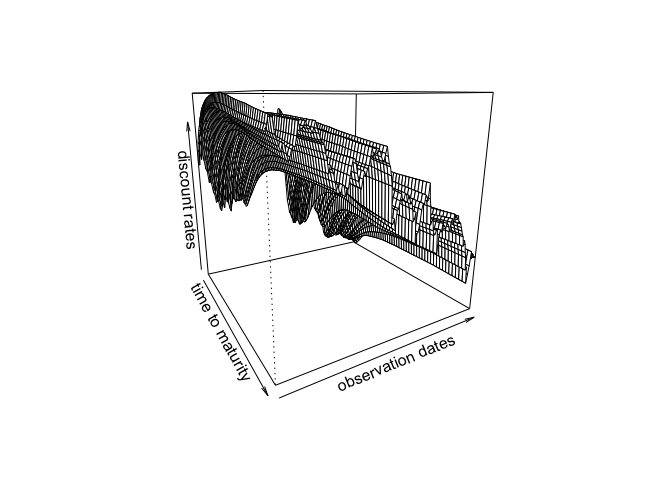
\includegraphics[width=14cm]{gfx/chapter-rvfl-mts/bundesbank_dR.png}
\caption{Observed discount rates from Deutsche Bundesbank website, from 2002 to the end 2015}
\label{db_zerorates}
\end{figure}

\begin{table}
\begin{center}
% table caption is above the table
\caption{Summary of observed discount rates from Deutsche Bundesbank website, from 2002 to the end 2015}
\label{tab:summary_db_zeros}       % Give a unique label
% For LaTeX tables use
\begin{tabular}{llllll}
\hline\noalign{\smallskip}
Maturity & Min & 1st Qrt  & Median  & 3rd Qrt  & Max  \\
\noalign{\smallskip}\hline\noalign{\smallskip}
  1 & -0.116 & 0.858 & 2.045 & 3.072 & 5.356 \\
  5 & 0.170 & 1.327 & 2.863 & 3.807 & 5.146\\
  15 & 0.711 & 2.616 & 3.954 & 4.702 & 5.758\\
  30 & 0.805 & 2.594 & 3.962 & 4.814 & 5.784\\
  50 & 0.749 & 2.647 & 3.630 & 4.590 & 5.467\\
\noalign{\smallskip}\hline
\end{tabular}
\end{center}
\end{table}

In the DNS framework, the spot interest rates observed at time $t$, for time to maturity $\tau$ are modeled as:
\begin{equation}
R_t(\tau) = \alpha_{1, t} + \alpha_{2, t}\left(\frac{1-e^{-\tau/\lambda}}{e^{-\tau/\lambda}}\right) + \alpha_{3, t}\left(\frac{1-e^{-\tau/\lambda}}{e^{-\tau/\lambda}} - e^{-\tau/\lambda}\right)
\end{equation}

\medskip

The factor loadings $1$, $\left(\frac{1-e^{-T/\lambda}}{e^{-T/\lambda}}\right)$ and $\left(\frac{1-e^{-T/\lambda}}{e^{-T/\lambda}} - e^{-T/\lambda}\right)$ are used to represent the level, slope, and curvature of the Yield Curve. We obtain estimations of $\alpha_{i, t}, i = 1, \ldots, 3$ for each cross-section of yields by fixing $\lambda$, and doing a least squares regression on the factor loadings. The three time series $\alpha_{i, t}, i = 1, \ldots, 3$ associated to the loadings for each cross-section of yields, are those that we wish to forecast simultaneously, by using an RVFL model.

\medskip

This type of model (DNS) cannot be used for no-arbitrage pricing as is, but it could be useful for example, for \textit{stressing} the yield curve factors under the historical probability. It can however be made arbitrage-free, if necessary (see \cite{diebold2013yield}). We will benchmark the RVFL model applied to the three time series $\alpha_{i, t}, i = 1, \ldots, 3$, against ARIMA and VAR models. \cite{diebold2006forecasting} applied an autoregressive AR(1) model separately to each one of the parameters, $\alpha_{i, t}, i = 1, \ldots, 3$. 

\medskip

We will apply to these parameters' series: an ARIMA model (\cite{hyndman2008automatic}), and a Vector Autoregressive model (VAR, see \cite{pfaff2008var} and \cite{lutkepohl2005new}); with the parameter $\lambda$ of the DNS factor loadings, used as an \textit{hyperparameter} for the time series cross-validation. In the RVFL and the VAR model, the number of lags is also used as an \textit{hyperparameter} for the cross-validation. For the RVFL, the most recent values of $\alpha_{i, t}, i = 1, \ldots, 3$ are stored in matrix $\bfY$, as described in section \ref{solve_rvfl}, ordered by \textit{date of arrival}, whereas matrix $\bfX$ contains the lags of the three series.

\medskip

A rolling forecasting methodology (see \cite{bergmeir2015note}) is implemented in order to obtain these benchmarks. A fixed 12 months-length window for training the model, and the following 12 months for testing, the origin of the training set is then advanced of 1 month, and the training/testing procedure is repeated. The measure of forecasting performance is the Root Mean Squared Error ($RMSE$).

\begin{figure}[!htb]
\centering
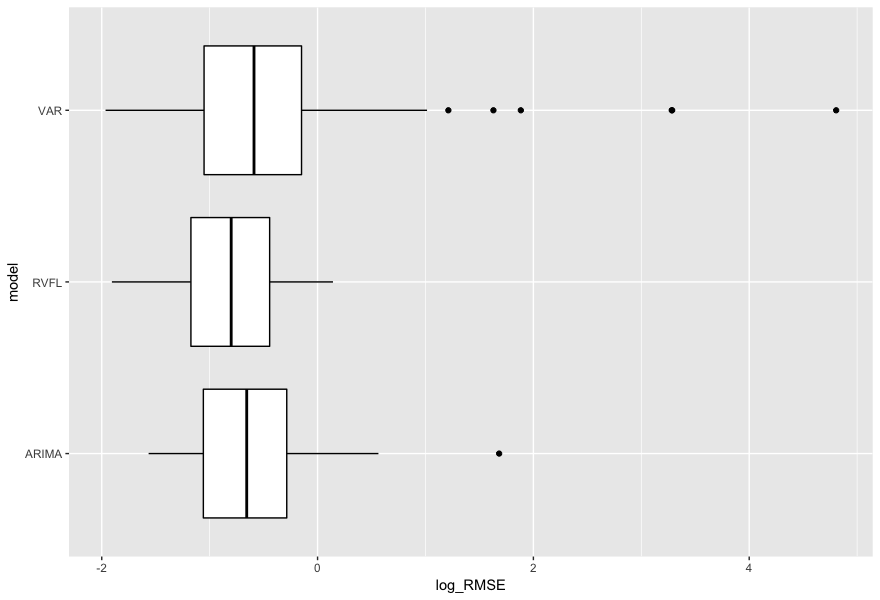
\includegraphics[width=10cm]{gfx/chapter-rvfl-mts/boxplot.png}
\caption{Distribution of out-of-sample $log(RMSE)$, for ARIMA, VAR, and RVFL}
\label{error_dist}
\end{figure}

\begin{figure}[!htb]
\centering
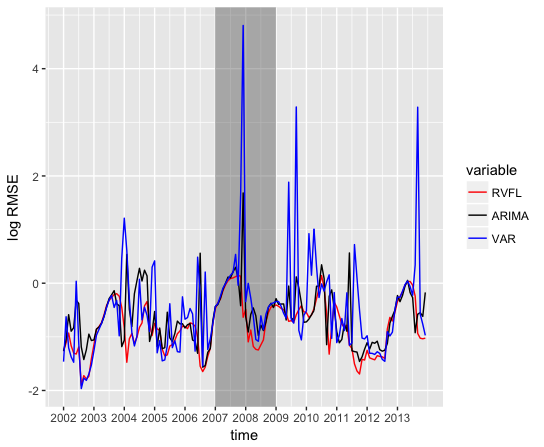
\includegraphics[width=10cm]{gfx/chapter-rvfl-mts/log_RMSE.png}
\caption{Out-of-sample $log(RMSE)$, for ARIMA, VAR, and RVFL over time}
\label{log_RMSE}
\end{figure}

Figure \ref{error_dist} presents boxplots for the distribution of out-of-sample errors obtained in the cross-validation procedure, and figure \ref{log_RMSE} presents the 12 months-ahead out-of-sample errors over time. ARIMA (separate (\cite{hyndman2008automatic}) ARIMA models applied to each series $\alpha_{i, t}, i = 1, \ldots, 3$) gives good results, as already suggested by  \cite{diebold2006forecasting}. They are nearly comparable to results from RVFL, but a bit more volatile, with an outlier point observed on the $log(RMSE)$ box plot. 

\medskip

The unrestricted VAR model results include more volatility than the two other methods on this specific  example, especially in the period of financial crisis going from 2007 to 2009, as seen on figure ~\ref{log_RMSE}. Table ~\ref{tab:benchmark} is to be read in conjuction with the $log(RMSE)$ box plot presented in figure ~\ref{error_dist}. It summarises the results obtained by the different methods on the out-of-sample $RMSE$. Table ~\ref{tab:confint} contains $95\%$ confidence intervals around the mean of the differences between the three methods.

\medskip

\begin{table}
\begin{center}
% table caption is above the table
\caption{Comparison of 12 months ahead out-of-sample $RMSE$, for the ARIMA, RVFL, and VAR}
\label{tab:benchmark}       % Give a unique label
% For LaTeX tables use
\begin{tabular}{lllllll}
\hline\noalign{\smallskip}
Method & Min & 1st Qrt  & Median & Mean  & 3rd Qrt  & Max  \\
\noalign{\smallskip}\hline\noalign{\smallskip}
  RVFL & 0.1487 & \textbf{0.3092} & \textbf{0.4491} & \textbf{0.5041} & \textbf{0.6414} & \textbf{1.1535} \\
  ARIMA & 0.2089 & 0.3470 & 0.5187 & 0.6358 & 0.7516 & 5.3798\\
  VAR & \textbf{0.1402} & 0.3493 & 0.5549 & 1.9522  & 0.8619 & 122.2214 \\
\noalign{\smallskip}\hline
\end{tabular}
\end{center}
\end{table}


\begin{table}
\begin{center}
% table caption is above the table
\caption{95\% confidence interval around the difference of out-of-sample $RMSE$}
\label{tab:confint}       % Give a unique label
% For LaTeX tables use
\begin{tabular}{lllllll}
\hline\noalign{\smallskip}
Method & Lower bound & Upper bound  & Mean \\
\noalign{\smallskip}\hline\noalign{\smallskip}
  RVFL - ARIMA & -0.2116 & -0.0518 & \textbf{-0.1317}\\
  RVFL - VAR & -3.1888 & 0.2927 & \textbf{-1.4480} \\
  ARIMA - VAR & -2.9937 & 0.3610 & \textbf{-1.3163} \\
\noalign{\smallskip}\hline
\end{tabular}
\end{center}
\end{table}

\medskip

Another advantage of RVFL over ARIMA or AR(1) in this context is that, it would be possible to add other variables to the RVFL regression, such as inflation, or dummy variables for external events, and combine their effects. It is also possible to stress one variable, and see the effects on the other variables, as presented in the appendix section \ref{fcst_ci}: the parameter $\alpha_{1, t}$ is increased (from $0.75$ to $1.25$) and decreased (from $0.75$ to $0.25$), and the other parameters $\alpha_{2, t}$ and $\alpha_{3, t}$ forecasts move slightly, consecutively to these \textit{stresses}. The corresponding median forecast curves for these stresses, and some additional ones, are presented in figure ~\ref{stressed_NS2}.

\begin{figure}
\centering
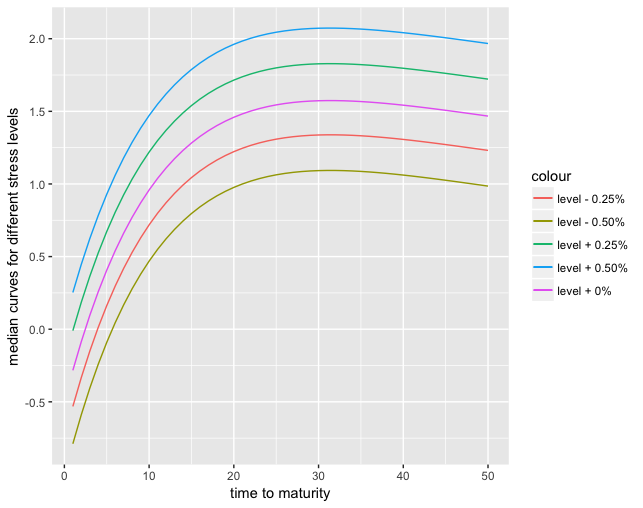
\includegraphics[width=11cm]{gfx/chapter-rvfl-mts/stressed_NS.png}
\caption{12 months-ahead median curves, for stressed yield curve level $\alpha_{1, t}$}
\label{stressed_NS2}
\end{figure}

\subsection{Forecasting 1 year, 10 years and 20 years spot rates}

For this second example, we forecast the 1-year, 10-years and 20-years spot rates time series from the previous dataset, on a 12-months horizon. As described in the previous section, we use a rolling forecasting methodology, with a training window of 12 months length. 

\medskip

Figure \ref{ex2_data} presents the three time series of data, and a summary of the data can be found in tables \ref{tab:three_ts} and \ref{tab:three_ts_cor}.

\begin{figure}
\centering
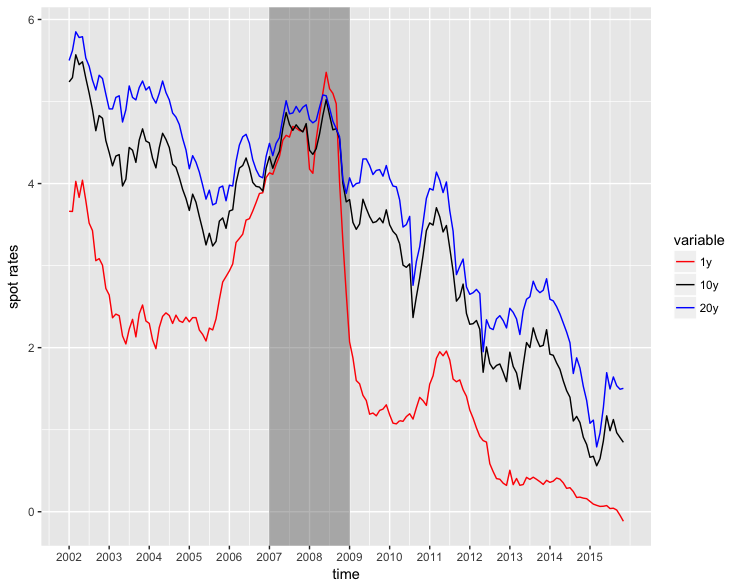
\includegraphics[width=12cm]{gfx/chapter-rvfl-mts/ex2_data.png}
\caption{1-year, 10-years and 20-years spot rates time series data}
\label{ex2_data}
\end{figure}

\begin{table}[!htb]
\begin{center}
% table caption is above the table
\caption{Summary of the data for 1 year, 10 years and 20 years spot rates time series (in \%)}
\label{tab:three_ts}       % Give a unique label
% For LaTeX tables use
\begin{tabular}{lllllll}
\hline\noalign{\smallskip}
Method & Min & 1st Qrt  & Median & Mean  & 3rd Qrt  & Max  \\
\noalign{\smallskip}\hline\noalign{\smallskip}
  1y rate & -0.116 & 0.858 & 2.045 & 2.062 & 3.072 & 5.356 \\
  10y rate & 0.560 & 2.221 & 3.581 & 3.322 & 4.354 & 5.570\\
  20y rate & 0.790 & 2.685 & 4.050 & 3.782 & 4.830 & 5.850\\
\noalign{\smallskip}\hline
\end{tabular}
\end{center}
\end{table}

\begin{table}[!htb]
\begin{center}
% table caption is above the table
\caption{Summary of data for 1 year, 10 years and 20 years spot rates time series}
\label{tab:three_ts_cor}       % Give a unique label
% For LaTeX tables use
\begin{tabular}{lllllll}
\hline\noalign{\smallskip}
Correlations & 1y rate & 10y rate  & 20y rate \\
\noalign{\smallskip}\hline\noalign{\smallskip}
  1y rate  & 1.0000  & 0.8729 & 0.8118\\
  10y rate & 0.8729 & 1.0000 & 0.9900 \\
  20y rate & 0.8118 & 0.9900 & 1.0000 \\
\noalign{\smallskip}\hline
\end{tabular}
\end{center}
\end{table}

The three time series globally exhibit a decreasing trend, and are highly positively correlated. The spot rates for short-term maturities can also be negative, as it has been observed recently in 2016. The spreads between the spot rates time series are extremely narrow during the 2007-2009 crisis. The tables below contain the results of a comparison between the RVFL model and an unrestricted VAR model (with one lag, \textit{best} parameter found) on the forecasting problem. The \textit{best} RVFL model, with the lowest out-of-sample $RMSE$, uses one lag, four hidden nodes, and $\lambda_1 = 5.80$, $\lambda_2 = 19.66$.

\begin{table}[!htb]
\begin{center}
% table caption is above the table
\caption{Comparison of 12 months ahead out-of-sample $RMSE$, for the RVFL, and VAR}
\label{tab:benchmark2}       % Give a unique label
% For LaTeX tables use
\begin{tabular}{lllllll}
\hline\noalign{\smallskip}
Method & Min & 1st Qrt  & Median & Mean  & 3rd Qrt  & Max  \\
\noalign{\smallskip}\hline\noalign{\smallskip}
  RVFL & 0.1675 & \textbf{0.2906} & \textbf{0.4704} & \textbf{0.5452} & \textbf{0.6469} & \textbf{1.8410} \\
  VAR &  \textbf{0.1382} & 0.4025 & 0.6469 & 1.0310 & 1.0750 & 13.020 \\
\noalign{\smallskip}\hline
\end{tabular}
\end{center}
\end{table}

\begin{table}[!htb]
\begin{center}
% table caption is above the table
\caption{95\% confidence interval around the difference of out-of-sample $RMSE$}
\label{tab:confint2}       % Give a unique label
% For LaTeX tables use
\begin{tabular}{lllllll}
\hline\noalign{\smallskip}
Method & Lower bound & Upper bound  & Mean \\
\noalign{\smallskip}\hline\noalign{\smallskip}
  RVFL-VAR & -0.2622 & -0.7087 & -\textbf{0.4854} \\
\noalign{\smallskip}\hline
\end{tabular}
\end{center}
\end{table}

\subsection{Forecasting on a longer horizon, with a longer training window}

In this third example, as in section \ref{section:dnsexample1}, we apply the DNS framework to the forecasting of spot rates. But with a longer training set (36 months), and a longer horizon for the test set (36 months as well). We use interest rate swaps data from the Federal Reserve Bank of St Louis website \footnote{Available at https://fred.stlouisfed.org/categories/32299}, observed on a monthly basis from july 2000 to september 2016, with maturities equal to $1, 2, 3, 4, 5, 7, 10, 30$, and a tenor equal to three months. 

\medskip

On figure \ref{example3:1}, we present three of the eight time series of swap rates, observed for time to maturities equal to $3, 10$ and $30$. The swap rates for different maturities generally exhibit a decreasing trend, and are nearly equal to 0 by the end of 2016, for the shortest maturities. 

\begin{figure}[!htb]
\centering
% Use the relevant command to insert your figure file.
% For example, with the graphicx package use
  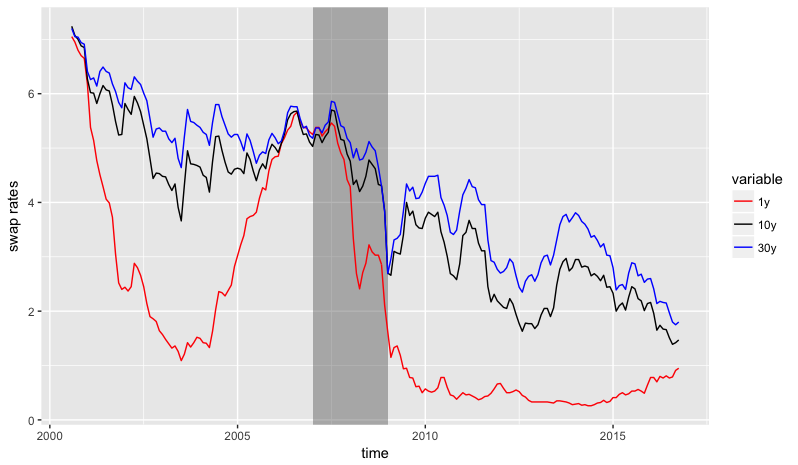
\includegraphics[width=14cm]{gfx/chapter-rvfl-mts/fredswaprates}
% figure caption is below the figure
\caption{Swap rates data (in \%) from St Louis Federal Reserve Bank, at maturities $1, 10, 30$}
\label{example3:1}       % Give a unique label
\end{figure}

\medskip

We also observe that the spreads between swap rates with different maturities start to narrow in 2006 until the end of 2007, and the  swap rates for short term maturities are relatively high during the same period. This is the period corresponding to the Liquidity and Credit Crunch 2007-2008. Table \ref{tab:freddatatables1} presents the descriptive statistics for these three time series. 

\begin{table}
\begin{center}
% table caption is above the table
\caption{Descriptive statistics of St Louis Federal Reserve data for 1y, 10y and 30y swap rates (in \%)}
\label{tab:freddatatables1}       % Give a unique label
% For LaTeX tables use
\begin{tabular}{lllllll}
\hline\noalign{\smallskip}
Maturity & Min. & 1st Qrt & Median & Mean & 3rd Qrt & Max.\\
\noalign{\smallskip}\hline\noalign{\smallskip}
  1  & 0.260 & 0.500  & 1.340  & 2.108  & 3.360  & 7.050\\
  10 & 1.390 & 2.610  & 4.190  & 3.881  & 5.020  & 7.240\\
  30 & 1.750 & 3.270  & 4.650  & 4.404  & 5.375  & 7.200\\
\noalign{\smallskip}\hline
\end{tabular}
\end{center}
\end{table}

\medskip

All the swap rates (for all the maturities available) were then transformed into zero rates, by using a single curve calibration methodology (that is, ignoring the counterparty credit risk) with linear interpolation between the swaps' maturities. Then, the Nelson \& Siegel model was used for fitting and forecasting the curves in a DNS framework, with both \code{auto.arima} and the RVFL model presented in this chapter, applied to the three factors. In the fashion of section ~\ref{section:dnsexample1}. But now, we obtain 36-months ahead forecasts, from a rolling training windows with a fixed 36 months length. The average out-of-sample $RMSE$ are then calculated for each method. 

\medskip

The \textit{best} hyperparameters - associated with the lowest out-of-sample average $RMSE$ - for each model are obtained through a search on a grid of values. We have:
\begin{itemize}
\item DNS with ARIMA (\code{auto.arima}): $\lambda = 1.4271$ (Nelson Siegel parameter)  
\item DNS with RVFL: \textbf{number of lags} for each series: 1, \textbf{activation function}: ReLU, \textbf{number of nodes} in the hidden layer: $45$, $\lambda_1 = 4.6416$, $\lambda_2 = 774.2637$ (RVFL parameters) and $\lambda = 24$ (Nelson Siegel parameter)   
\end{itemize}

\medskip

With these parameters, the results detailed in table \ref{tab:freddatatables4} are obtained, for the out-of-sample $RMSE$. A $95\%$ confidence interval around the difference of out-of-sample $RMSE$ between ARIMA (applied to each one of the three factors) and RVFL is presented in table \ref{tab:confint3}. 

\begin{table}[!htb]
\begin{center}
% table caption is above the table
\caption{Descriptive statistics for out-of-sample $RMSE$, with rolling training window = 36 months, and testing window = 36 months}
\label{tab:freddatatables4}       % Give a unique label
% For LaTeX tables use
\begin{tabular}{llllllll}
\hline\noalign{\smallskip}
Method & Min. & 1st Qrt & Median & Mean & 3rd Qrt & Max. & Std. Dev\\
\noalign{\smallskip}\hline\noalign{\smallskip}
  ARIMA   & 0.0036  & \textbf{0.0070}  & \textbf{0.0104}  & 0.0149  & 0.0161  & 0.2150 & 0.0213\\
  RVFL    & \textbf{0.0032}  & 0.0078  & 0.0115  & \textbf{0.0120}  & \textbf{0.0148}  & \textbf{0.0256} & \textbf{0.0055}\\
\noalign{\smallskip}\hline
\end{tabular}
\end{center}
\end{table}

\begin{table}[!htb]
\begin{center}
% table caption is above the table
\caption{95\% confidence interval around the difference of out-of-sample $RMSE$}
\label{tab:confint3}       % Give a unique label
% For LaTeX tables use
\begin{tabular}{lllllll}
\hline\noalign{\smallskip}
Method & Lower bound & Upper bound  & Mean \\
\noalign{\smallskip}\hline\noalign{\smallskip}
  RVFL-ARIMA & -0.0064 & 0.0007 & \textbf{-0.0028} \\
\noalign{\smallskip}\hline
\end{tabular}
\end{center}
\end{table}

Figure \ref{example3:2} presents the evolution of the out-of-sample $log(RMSE)$ over the training/testing windows. The grey rectangle indicating the Liquidity and Credit crunch is larger here, because in this example, a training set starting in 2004 has its test set starting 36 months later, in 2007. Again, we observe that the results from the RVFL model exhibit a low out-of-sample error, along with a low volatility.

\begin{figure}[!htb]
\centering
% Use the relevant command to insert your figure file.
% For example, with the graphicx package use
  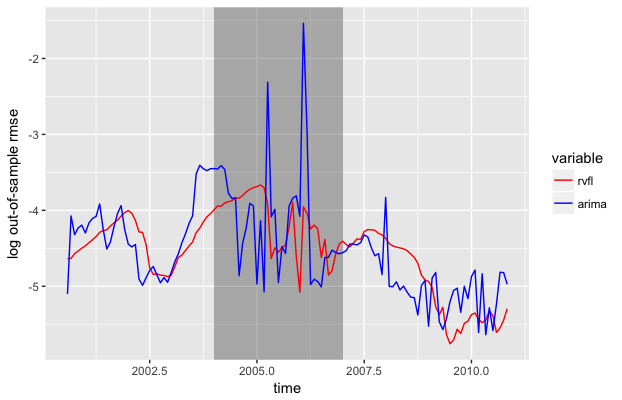
\includegraphics[width=14cm]{gfx/chapter-rvfl-mts/log_oos_rmse_rvfl_arima}
% figure caption is below the figure
\caption{Out-of-sample $log(RMSE)$, for ARIMA and RVFL over time}
\label{example3:2}       % Give a unique label
\end{figure}

\medskip

Figure \ref{example3:3}, presents the convergence of the out-of-sample $log(RMSE)$ for the DNS + RVFL model from this section, as a function of $log(\lambda_1)$ and $log(\lambda_2)$. $\lambda_1$ and $\lambda_2$ both range from $10^{-2}$ to $10^{4}$, with ten equally-spaced points each (hence, a grid of one hundred points $\left( log(\lambda_1), log(\lambda_2), log(RMSE)\right)$. 

\medskip

The number of nodes in the hidden layer is equal to $45$, and the value of $\lambda$, parameter from the \cite{nelson1987parsimonious} model presented in section \ref{section:dnsexample1}, is fixed and equal to $24$. The one hundred points $\left( log(\lambda_1), log(\lambda_2), log(RMSE)\right)$ that we use for figure \ref{example3:3} can be found in appendix \ref{sec:cv_log_rmse}. 

\medskip

There is a rectangular region at the top, in the middle of the figure, where the $log(RMSE)$ is the lowest. In this region, the lowest value of the out-of-sample $log(RMSE)$ is observed for $\lambda_1 = 4.6416$ and $\lambda_2 = 464.1589$ and the out-of-sample $RMSE$ is equal to $0.01206$ ($75^{th}$ point in appendix \ref{sec:cv_log_rmse}).   

\begin{figure}[!htb]
\centering
% Use the relevant command to insert your figure file.
% For example, with the graphicx package use
  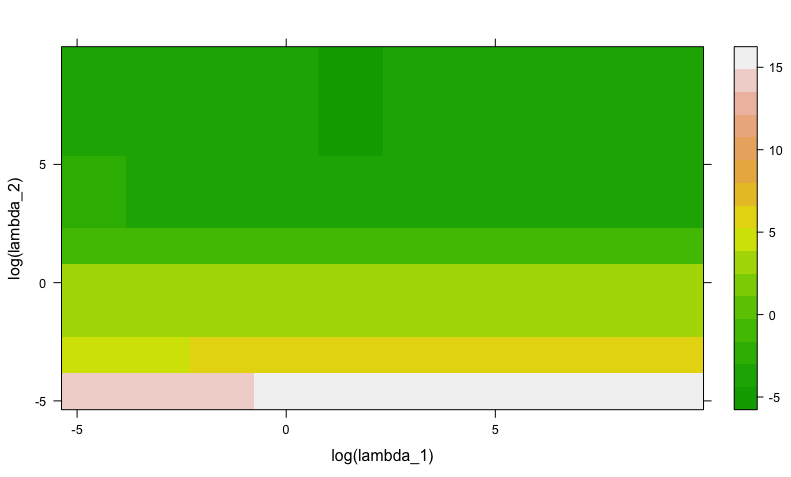
\includegraphics[width=14cm]{gfx/chapter-rvfl-mts/log_rmse_convergence}
% figure caption is below the figure
\caption{Out-of-sample $log(RMSE)$, as a function of $\lambda_1$ and $\lambda_2$}
\label{example3:3}       % Give a unique label
\end{figure}

\newpage

\section{Conclusion}

We present a model which could be used for multiple time series forecasting, based on a single layer quasi-randomized neural network. In this model, the lags of the different time series are used as in a dynamic regression model, and include the response variable lags. An additional layer of variables is added to the regression, whose nodes are not trained but obtained from a low discrepancy sequence. It is possible to add new variables to the regression, as indicators of special events, or to stress one variable, and observe the implied effect on the others' forecast. The model is tested on raw historical spot rates, and in a Dynamic Nelson Siegel framework. It produces \textit{robust} forecast results when compared to other usual (unpenalized) models in the same framework.

\newpage

\section{Appendix}

\subsection{Mean forecast and confidence intervals for $\alpha_{i, t}, i = 1, \ldots, 3$ forecasts}
\label{fcst_ci}

$\alpha_{1, t}$:

\begin{verbatim}
alpha1    y_lo80    y_hi80    y_lo95    y_hi95
13 0.7432724 0.6852024 0.8013425 0.6544620 0.8320829
14 0.7357374 0.6776673 0.7938074 0.6469269 0.8245478
15 0.7378042 0.6797342 0.7958742 0.6489938 0.8266147
16 0.7408417 0.6827717 0.7989118 0.6520313 0.8296522
17 0.7407904 0.6827204 0.7988604 0.6519800 0.8296009
18 0.7404501 0.6823801 0.7985201 0.6516396 0.8292605
19 0.7403603 0.6822903 0.7984303 0.6515498 0.8291707
20 0.7403981 0.6823281 0.7984681 0.6515876 0.8292085
21 0.7404788 0.6824087 0.7985488 0.6516683 0.8292892
22 0.7404786 0.6824086 0.7985487 0.6516682 0.8292891
23 0.7404791 0.6824091 0.7985491 0.6516686 0.8292895
24 0.7404758 0.6824058 0.7985458 0.6516654 0.8292863
\end{verbatim}

$\alpha_{2, t}$:

\begin{verbatim}
 alpha2    y_lo80    y_hi80    y_lo95    y_hi95
13 -1.250640 -1.351785 -1.149495 -1.405328 -1.095952
14 -1.243294 -1.344439 -1.142149 -1.397982 -1.088606
15 -1.241429 -1.342574 -1.140284 -1.396117 -1.086741
16 -1.243868 -1.345014 -1.142723 -1.398557 -1.089180
17 -1.244483 -1.345628 -1.143338 -1.399171 -1.089795
18 -1.241865 -1.343010 -1.140719 -1.396553 -1.087177
19 -1.240814 -1.341959 -1.139669 -1.395502 -1.086126
20 -1.240371 -1.341516 -1.139226 -1.395059 -1.085683
21 -1.240237 -1.341382 -1.139092 -1.394925 -1.085549
22 -1.240276 -1.341421 -1.139131 -1.394964 -1.085588
23 -1.240329 -1.341474 -1.139184 -1.395017 -1.085641
24 -1.240308 -1.341453 -1.139163 -1.394996 -1.085620
\end{verbatim}

$\alpha_{3, t}$:

\begin{verbatim}
 alpha3   y_lo80   y_hi80   y_lo95   y_hi95
13 4.584836 4.328843 4.757406 4.215410 4.870840
14 4.546167 4.307253 4.849862 4.163634 4.993482
15 4.527651 4.201991 4.803004 4.042913 4.962082
16 4.513810 4.216525 4.850160 4.048812 5.017874
17 4.517643 4.176214 4.828735 4.003502 5.001446
18 4.523109 4.203064 4.866713 4.027406 5.042371
19 4.522772 4.178489 4.848760 4.001079 5.026170
20 4.521846 4.191833 4.866066 4.013374 5.044524
21 4.521382 4.177560 4.854171 3.998472 5.033259
22 4.521451 4.186714 4.864755 4.007248 5.044222
23 4.521772 4.178995 4.857897 3.999300 5.037591
24 4.521862 4.184734 4.864155 4.004903 5.043987
\end{verbatim}

\subsection{Stressed forecast ($\alpha_{1, t} + 0.5\%$) and confidence intervals for $\alpha_{i, t}, i = 1, \ldots, 3$ forecasts}

$\alpha_{1, t}$:

\begin{verbatim}
 alpha1  y_lo80  y_hi80  y_lo95  y_hi95
13   1.25 1.19193 1.30807 1.16119 1.33881
14   1.25 1.19193 1.30807 1.16119 1.33881
15   1.25 1.19193 1.30807 1.16119 1.33881
16   1.25 1.19193 1.30807 1.16119 1.33881
17   1.25 1.19193 1.30807 1.16119 1.33881
18   1.25 1.19193 1.30807 1.16119 1.33881
19   1.25 1.19193 1.30807 1.16119 1.33881
20   1.25 1.19193 1.30807 1.16119 1.33881
21   1.25 1.19193 1.30807 1.16119 1.33881
22   1.25 1.19193 1.30807 1.16119 1.33881
23   1.25 1.19193 1.30807 1.16119 1.33881
24   1.25 1.19193 1.30807 1.16119 1.33881
\end{verbatim}

$\alpha_{2, t}$:

\begin{verbatim}
 alpha2    y_lo80    y_hi80    y_lo95    y_hi95
13 -1.222568 -1.323713 -1.121423 -1.377256 -1.067880
14 -1.219401 -1.320546 -1.118256 -1.374089 -1.064713
15 -1.211361 -1.312506 -1.110216 -1.366049 -1.056673
16 -1.216213 -1.317358 -1.115068 -1.370901 -1.061525
17 -1.215266 -1.316411 -1.114121 -1.369954 -1.060578
18 -1.211474 -1.312619 -1.110329 -1.366162 -1.056786
19 -1.210329 -1.311474 -1.109183 -1.365017 -1.055640
20 -1.209610 -1.310755 -1.108465 -1.364298 -1.054922
21 -1.209648 -1.310793 -1.108503 -1.364336 -1.054960
22 -1.209601 -1.310746 -1.108456 -1.364289 -1.054913
23 -1.209688 -1.310833 -1.108542 -1.364376 -1.055000
24 -1.209653 -1.310798 -1.108508 -1.364341 -1.054965
\end{verbatim}

$\alpha_{3, t}$:

\begin{verbatim}
alpha3   y_lo80   y_hi80   y_lo95   y_hi95
13 4.500390 4.244398 4.672961 4.130964 4.786394
14 4.482948 4.244035 4.786643 4.100415 4.930263
15 4.441841 4.116182 4.717194 3.957103 4.876272
16 4.441744 4.144459 4.778094 3.976746 4.945808
17 4.439609 4.098181 4.750701 3.925469 4.923413
18 4.447151 4.127105 4.790755 3.951448 4.966412
19 4.446164 4.101881 4.772152 3.924471 4.949562
20 4.445421 4.115407 4.789641 3.936949 4.968099
21 4.445411 4.101589 4.778200 3.922501 4.957289
22 4.445491 4.110754 4.788795 3.931287 4.968262
23 4.445937 4.103160 4.782062 3.923465 4.961756
24 4.446012 4.108885 4.788306 3.929053 4.968137
\end{verbatim}

\newpage

\nocite{dutang2015}
\nocite{wickham2016ggplot2}


\appendix

\subsection{Mean forecast and confidence intervals for $\alpha_{i, t}, i = 1, \ldots, 3$ forecasts}

$\alpha_{1, t}$:

\begin{verbatim}
alpha1    y_lo80    y_hi80    y_lo95    y_hi95
13 0.7432724 0.6852024 0.8013425 0.6544620 0.8320829
14 0.7357374 0.6776673 0.7938074 0.6469269 0.8245478
15 0.7378042 0.6797342 0.7958742 0.6489938 0.8266147
16 0.7408417 0.6827717 0.7989118 0.6520313 0.8296522
17 0.7407904 0.6827204 0.7988604 0.6519800 0.8296009
18 0.7404501 0.6823801 0.7985201 0.6516396 0.8292605
19 0.7403603 0.6822903 0.7984303 0.6515498 0.8291707
20 0.7403981 0.6823281 0.7984681 0.6515876 0.8292085
21 0.7404788 0.6824087 0.7985488 0.6516683 0.8292892
22 0.7404786 0.6824086 0.7985487 0.6516682 0.8292891
23 0.7404791 0.6824091 0.7985491 0.6516686 0.8292895
24 0.7404758 0.6824058 0.7985458 0.6516654 0.8292863
\end{verbatim}

$\alpha_{2, t}$:

\begin{verbatim}
 alpha2    y_lo80    y_hi80    y_lo95    y_hi95
13 -1.250640 -1.351785 -1.149495 -1.405328 -1.095952
14 -1.243294 -1.344439 -1.142149 -1.397982 -1.088606
15 -1.241429 -1.342574 -1.140284 -1.396117 -1.086741
16 -1.243868 -1.345014 -1.142723 -1.398557 -1.089180
17 -1.244483 -1.345628 -1.143338 -1.399171 -1.089795
18 -1.241865 -1.343010 -1.140719 -1.396553 -1.087177
19 -1.240814 -1.341959 -1.139669 -1.395502 -1.086126
20 -1.240371 -1.341516 -1.139226 -1.395059 -1.085683
21 -1.240237 -1.341382 -1.139092 -1.394925 -1.085549
22 -1.240276 -1.341421 -1.139131 -1.394964 -1.085588
23 -1.240329 -1.341474 -1.139184 -1.395017 -1.085641
24 -1.240308 -1.341453 -1.139163 -1.394996 -1.085620
\end{verbatim}

$\alpha_{3, t}$:

\begin{verbatim}
 alpha3   y_lo80   y_hi80   y_lo95   y_hi95
13 4.584836 4.328843 4.757406 4.215410 4.870840
14 4.546167 4.307253 4.849862 4.163634 4.993482
15 4.527651 4.201991 4.803004 4.042913 4.962082
16 4.513810 4.216525 4.850160 4.048812 5.017874
17 4.517643 4.176214 4.828735 4.003502 5.001446
18 4.523109 4.203064 4.866713 4.027406 5.042371
19 4.522772 4.178489 4.848760 4.001079 5.026170
20 4.521846 4.191833 4.866066 4.013374 5.044524
21 4.521382 4.177560 4.854171 3.998472 5.033259
22 4.521451 4.186714 4.864755 4.007248 5.044222
23 4.521772 4.178995 4.857897 3.999300 5.037591
24 4.521862 4.184734 4.864155 4.004903 5.043987
\end{verbatim}

\subsection{Stressed forecast ($\alpha_{1, t} + 0.5\%$) and confidence intervals for $\alpha_{i, t}, i = 1, \ldots, 3$ forecasts}

$\alpha_{1, t}$:

\begin{verbatim}
 alpha1  y_lo80  y_hi80  y_lo95  y_hi95
13   1.25 1.19193 1.30807 1.16119 1.33881
14   1.25 1.19193 1.30807 1.16119 1.33881
15   1.25 1.19193 1.30807 1.16119 1.33881
16   1.25 1.19193 1.30807 1.16119 1.33881
17   1.25 1.19193 1.30807 1.16119 1.33881
18   1.25 1.19193 1.30807 1.16119 1.33881
19   1.25 1.19193 1.30807 1.16119 1.33881
20   1.25 1.19193 1.30807 1.16119 1.33881
21   1.25 1.19193 1.30807 1.16119 1.33881
22   1.25 1.19193 1.30807 1.16119 1.33881
23   1.25 1.19193 1.30807 1.16119 1.33881
24   1.25 1.19193 1.30807 1.16119 1.33881
\end{verbatim}

$\alpha_{2, t}$:

\begin{verbatim}
 alpha2    y_lo80    y_hi80    y_lo95    y_hi95
13 -1.222568 -1.323713 -1.121423 -1.377256 -1.067880
14 -1.219401 -1.320546 -1.118256 -1.374089 -1.064713
15 -1.211361 -1.312506 -1.110216 -1.366049 -1.056673
16 -1.216213 -1.317358 -1.115068 -1.370901 -1.061525
17 -1.215266 -1.316411 -1.114121 -1.369954 -1.060578
18 -1.211474 -1.312619 -1.110329 -1.366162 -1.056786
19 -1.210329 -1.311474 -1.109183 -1.365017 -1.055640
20 -1.209610 -1.310755 -1.108465 -1.364298 -1.054922
21 -1.209648 -1.310793 -1.108503 -1.364336 -1.054960
22 -1.209601 -1.310746 -1.108456 -1.364289 -1.054913
23 -1.209688 -1.310833 -1.108542 -1.364376 -1.055000
24 -1.209653 -1.310798 -1.108508 -1.364341 -1.054965
\end{verbatim}

$\alpha_{3, t}$:

\begin{verbatim}
alpha3   y_lo80   y_hi80   y_lo95   y_hi95
13 4.500390 4.244398 4.672961 4.130964 4.786394
14 4.482948 4.244035 4.786643 4.100415 4.930263
15 4.441841 4.116182 4.717194 3.957103 4.876272
16 4.441744 4.144459 4.778094 3.976746 4.945808
17 4.439609 4.098181 4.750701 3.925469 4.923413
18 4.447151 4.127105 4.790755 3.951448 4.966412
19 4.446164 4.101881 4.772152 3.924471 4.949562
20 4.445421 4.115407 4.789641 3.936949 4.968099
21 4.445411 4.101589 4.778200 3.922501 4.957289
22 4.445491 4.110754 4.788795 3.931287 4.968262
23 4.445937 4.103160 4.782062 3.923465 4.961756
24 4.446012 4.108885 4.788306 3.929053 4.968137
\end{verbatim}

\subsection{Out-of-sample $log(RMSE)$ as a function of $log(\lambda_1)$ and $log(\lambda_2)$}
\label{sec:cv_log_rmse}

\begin{verbatim}
    log_lambda1 log_lambda2  log_error
1     -4.605170   -4.605170 13.5039336
2     -3.070113   -4.605170 14.3538621
3     -1.535057   -4.605170 14.7912525
4      0.000000   -4.605170 14.8749375
5      1.535057   -4.605170 14.8928025
6      3.070113   -4.605170 14.8962203
7      4.605170   -4.605170 14.8975776
8      6.140227   -4.605170 14.8976494
9      7.675284   -4.605170 14.8976630
10     9.210340   -4.605170 14.8976715
11    -4.605170   -3.070113  3.9701229
12    -3.070113   -3.070113  4.9644144
13    -1.535057   -3.070113  5.2607788
14     0.000000   -3.070113  5.3208833
15     1.535057   -3.070113  5.3326856
16     3.070113   -3.070113  5.3351784
17     4.605170   -3.070113  5.3357136
18     6.140227   -3.070113  5.3358306
19     7.675284   -3.070113  5.3358557
20     9.210340   -3.070113  5.3358610
21    -4.605170   -1.535057  3.6692928
22    -3.070113   -1.535057  3.5643607
23    -1.535057   -1.535057  3.5063072
24     0.000000   -1.535057  3.4942438
25     1.535057   -1.535057  3.4904354
26     3.070113   -1.535057  3.4881352
27     4.605170   -1.535057  3.4888202
28     6.140227   -1.535057  3.4880668
29     7.675284   -1.535057  3.4886911
30     9.210340   -1.535057  3.4886383
31    -4.605170    0.000000  3.6224691
32    -3.070113    0.000000  3.8313407
33    -1.535057    0.000000  3.8518759
34     0.000000    0.000000  3.8163287
35     1.535057    0.000000  3.7993471
36     3.070113    0.000000  3.7948073
37     4.605170    0.000000  3.7937787
38     6.140227    0.000000  3.7935546
39     7.675284    0.000000  3.7935063
40     9.210340    0.000000  3.7934958
41    -4.605170    1.535057 -1.2115597
42    -3.070113    1.535057 -1.0130537
43    -1.535057    1.535057 -0.5841784
44     0.000000    1.535057 -0.3802817
45     1.535057    1.535057 -0.3109827
46     3.070113    1.535057 -0.2931830
47     4.605170    1.535057 -0.2891586
48     6.140227    1.535057 -0.2882824
49     7.675284    1.535057 -0.2880932
50     9.210340    1.535057 -0.2880524
51    -4.605170    3.070113 -2.0397856
52    -3.070113    3.070113 -3.1729003
53    -1.535057    3.070113 -3.8655596
54     0.000000    3.070113 -3.9279840
55     1.535057    3.070113 -3.9508440
56     3.070113    3.070113 -4.0270316
57     4.605170    3.070113 -4.0831569
58     6.140227    3.070113 -4.0953167
59     7.675284    3.070113 -4.0979447
60     9.210340    3.070113 -4.0985113
61    -4.605170    4.605170 -2.6779260
62    -3.070113    4.605170 -3.4704808
63    -1.535057    4.605170 -4.0404935
64     0.000000    4.605170 -4.2441836
65     1.535057    4.605170 -4.3657802
66     3.070113    4.605170 -4.3923094
67     4.605170    4.605170 -4.3862826
68     6.140227    4.605170 -4.3830293
69     7.675284    4.605170 -4.3820703
70     9.210340    4.605170 -4.3818486
71    -4.605170    6.140227 -3.5007058
72    -3.070113    6.140227 -3.8389274
73    -1.535057    6.140227 -4.1969545
74     0.000000    6.140227 -4.3400025
75     1.535057    6.140227 -4.4179718
76     3.070113    6.140227 -4.3797034
77     4.605170    6.140227 -4.3073100
78     6.140227    6.140227 -4.2866647
79     7.675284    6.140227 -4.2820357
80     9.210340    6.140227 -4.2810151
81    -4.605170    7.675284 -3.7236774
82    -3.070113    7.675284 -4.0057353
83    -1.535057    7.675284 -4.2699684
84     0.000000    7.675284 -4.3569254
85     1.535057    7.675284 -4.4156364
86     3.070113    7.675284 -4.3842360
87     4.605170    7.675284 -4.2759516
88     6.140227    7.675284 -4.2425876
89     7.675284    7.675284 -4.2346514
90     9.210340    7.675284 -4.2328863
91    -4.605170    9.210340 -3.7706268
92    -3.070113    9.210340 -4.0406387
93    -1.535057    9.210340 -4.2776907
94     0.000000    9.210340 -4.3498230
95     1.535057    9.210340 -4.4095778
96     3.070113    9.210340 -4.3860089
97     4.605170    9.210340 -4.2647179
98     6.140227    9.210340 -4.2273624
99     7.675284    9.210340 -4.2183911
100    9.210340    9.210340 -4.2163638
\end{verbatim}

